%  Field_Modelling.tex
% !TeX spellcheck = en_GB
% !TeX root = ReportMain.tex

\section{Modelling Results} \label{s:model}
The following simulations were completed using the COMSOL multiphysics software package.
COMSOL is a professional finite element simulation package able to model a variety of physical features.
The following models are created using the AC/DC module, which is used to simulate electric and magnetic fields \cite{ComsolACDC}.
Specifically, the electrostatics interface is used. 
This solves a charge conservation equation for a given voltage and spacial distribution of charge \cite{ComsolACDC}.



\subsection{Finite Element Methods (FEM)}
There are inherent difficulties in solving the partial differential equations that govern many practical engineering problems \cite{kuffel2000high}.
Despite knowing the equations and appropriate boundary conditions that govern a problem, many are complicated by irregular geometries or other discontinuities.
Numerical methods allow approximate solutions to be obtained for problems intractable by analytic methods \cite{meshkatoddini2006study}.
In an analytic solution, the whole system is governed by a mathematical equation valid for the entire region of interest. 
Although these differential equations are often mathematically compact, it is difficult to obtain an answer unless the system is unreasonably simplified \cite{meshkatoddini2006study}.
In FEMs, the complex geometry is broken into a series of much smaller and simpler geometries \cite{kuffel2000high}.
These geometries can be squares, rectangles or triangles in 2D or the 3D equivalent shapes. 
These simpler shapes form interconnected subregions for which an approximate function, usually a high order polynomial, can be used to represent the actual function.
If the complex geometry is split into an adequate number of simple shapes, these approximate functions closely matches the exact solution \cite{meshkatoddini2006study}.

By default COMSOL uses a triangular discretisation to split up a complex geometry in a process called meshing.
This forms an unstructured grid of triangles, allowing the mapping of complex or curved geometries.
Other numerical methods such as Finite Difference Methods require a structured grid, hence FEMs are more flexible with regards to geometry \cite{kuffel2000high}.
Meshing requires an initial understanding of the expected outcomes of the problem, so that the mesh can be refined in areas of interest.
Each triangular element is approximated by a linear interpolation of the potential at the vertices of the triangle. 
A set of linear algebraic equations are formed by minimising the error between the actual solution and a set of approximate linear trial functions \cite{meshkatoddini2006study}.

\subsection{Equation Derivation and Boundary Conditions}
The electrostatics interface of the AC/DC COMSOL module uses the electric potential $V$ to calculate static electric fields.
A Poisson type partial differential equation is derived using classical electrostatics and Gauss' Law \cite{hayt2012engineering}.

By taking Gauss's Law:
\begin{equation}
\nabla.\mathbf{D} = \rho v
\end{equation}
the equation for electric flux density $\mathbf{D}$:
\begin{equation}
\mathbf{D} = \epsilon_0\epsilon_r\mathbf{E}
\end{equation}
this can be combined with the equation for a static electric field:
\begin{equation}
\mathbf{E} = -\nabla V
\end{equation}
to give by substitution:
\begin{equation}
\nabla.\mathbf{D} = \nabla.(\epsilon_0 \epsilon_r \mathbf{E}) = -\nabla.(\epsilon_0 \epsilon_r \nabla V) = \rho v
\end{equation}
which is more usually written:
\begin{equation}
\nabla^{2}V = -\frac{\rho v}{\epsilon_0 \epsilon_r}
\end{equation}
where $\epsilon_0$ is the permittivity of free space, $\epsilon_r$ is the relative permittivity of the material, $\mathbf{E}$ is the electric field strength and $\rho v$ is the volume charge density.

In the special case where there is zero volume charge density, that is $\rho v = 0$ then the equation simplifies to Laplace's Equation:
\begin{equation}
\nabla^{2}V = 0
\end{equation}

The models used in this paper are 2D axisymmetric, meaning that a 2D model is used to describe a 3D object that can be rotated $360^o$ about a central point $r=0$ to give a 3D geometry.
This assumes that not only is the geometry the same in the angular $\varphi$ direction, but also that the electric potential is constant.
In this case, Poissons equation can be rewritten in cylindrical coordinates for a 2D axisymmetric model, it is multiplied by r to ensure there are no singularities at $r=0$ \cite{meshkatoddini2006study}.
\begin{equation}
\begin{bmatrix} 
\displaystyle \frac{\partial}{\partial r} \\
\displaystyle\frac{\partial}{\partial z}
\end{bmatrix}^T
.(r \begin{bmatrix}
\displaystyle\frac{\partial V}{\partial r} \\
\displaystyle\frac{\partial V}{\partial z}
\end{bmatrix})
= -\displaystyle\frac{r\rho v}{\epsilon_0 \epsilon_r}
\end{equation}

The boundary conditions are defined as the following:
\begin{enumerate}
\item All boundaries with the conductor and with foil 0 are set to $V = V_0 = 275kV$
\item All boundaries with the transformer wall and with the outermost foil are set to $V = 0$
\item The interface between two insulator sub-domains is defined by $n.(\mathbf{D}_{1} -\mathbf{D}_{2}) = \rho v$ and $n\times(\mathbf{E}_{1} -\mathbf{E}_{2}) = 0$. These equations specify that the normal component of the electric flux density is discontinuous at the interface between two dielectrics, and that the tangential component of the electric field is continuous across the dielectric interface. $n$ is the normal outward vector pointing from dielectric 2 to dielectric 1.
\end{enumerate}

\subsection{Workflow}
In order to simulate the electric field distribution within our bushing design, 2D axisymmetric models were created. The general workflow to achieve this is:
\begin{enumerate}
\item Build a geometry representing the physical structure of the bushing.
\item Assign each geometric domain a material. The material selection determines the relative permittivity $\epsilon_r$ of each domain.
\item Define the charge conservation equation and all initial conditions. This includes setting which boundaries are at ground and conductor potential and setting boundary conditions.
\item Design a mesh. The geometry is split into smaller elements in order to compute the charge conservation equation. For designs with foils, special meshing parameters are required to speed up the process.
\item Carry out the study. This stage is the actual computation of the solution.
\item Post-processing. Display the results in a number of formats including 3D, 2D and 1D plots, or export the data for post-processing in Matlab.
\end{enumerate}


\subsection{Baseline Model}
In order to minimise the computation time required for each model, it was necessary to determine the areas of interest in the model.
A bushing geometry was built with no foils inserted. 
A high quality mesh was produced and the system was solved to find the electric field distribution throughout the bushing and the surrounding area.
\begin{figure}[!h]
  \centering
    \includegraphics[width = 0.8\textwidth]{./Figures/Simulations/Edited_No_Foils_Large/Geometry.eps} 
\caption{Baseline Model Geometry}
\label{Figure:No_Foil_Large_Geom}
\end{figure}

\begin{figure}[!h]
  \centering
    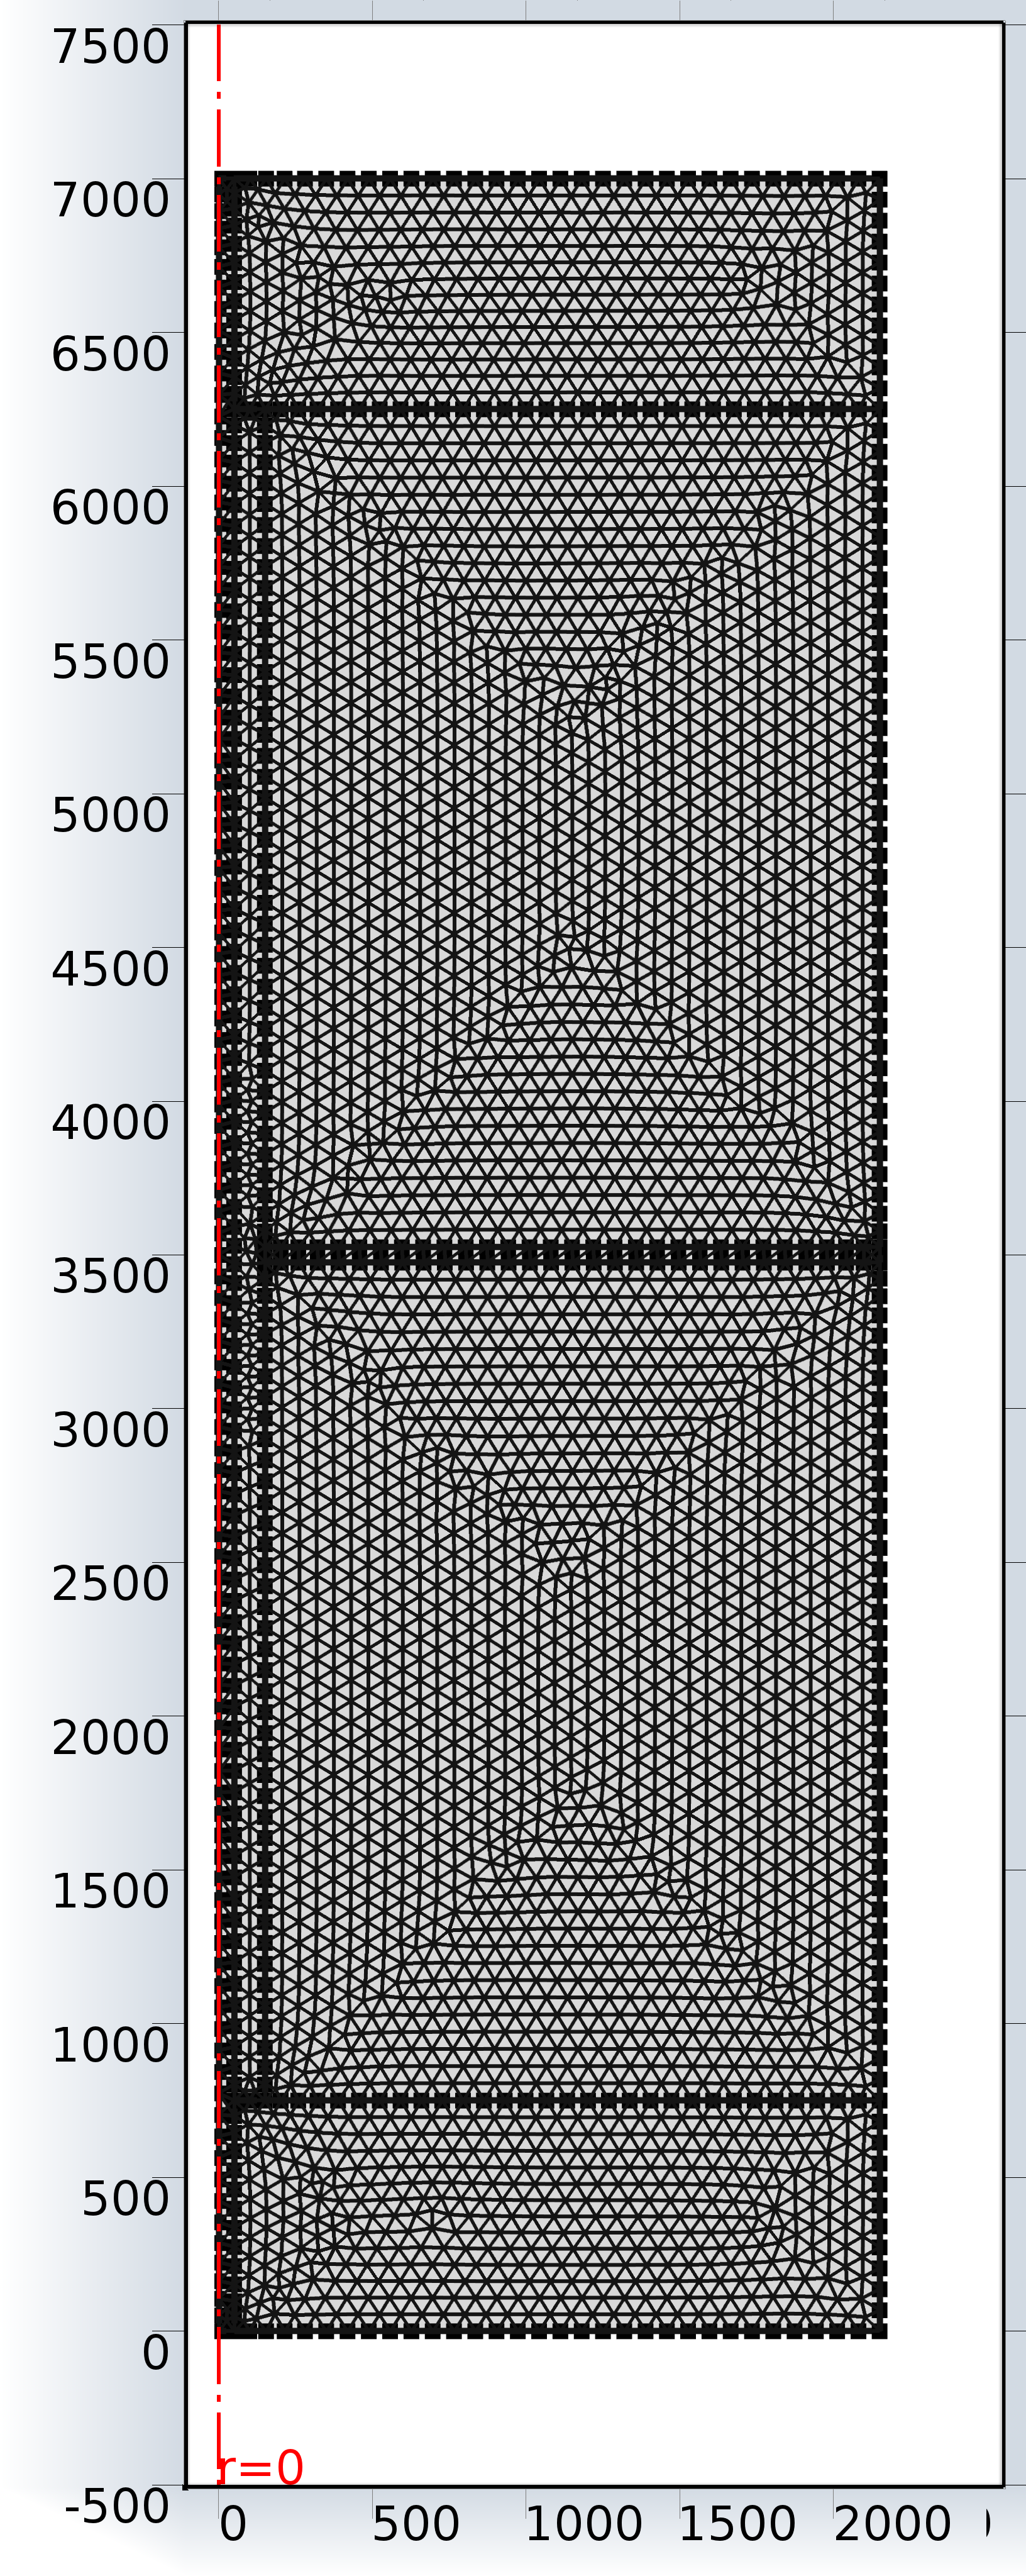
\includegraphics[width = 0.8\textwidth]{./Figures/Simulations/Edited_No_Foils_Large/Meshing.eps} 
\caption{Extra Fine Meshing for Baseline Model}
\label{Figure:No_Foil_Large_Mesh}
\end{figure}

\begin{figure}[!h]
  \centering
    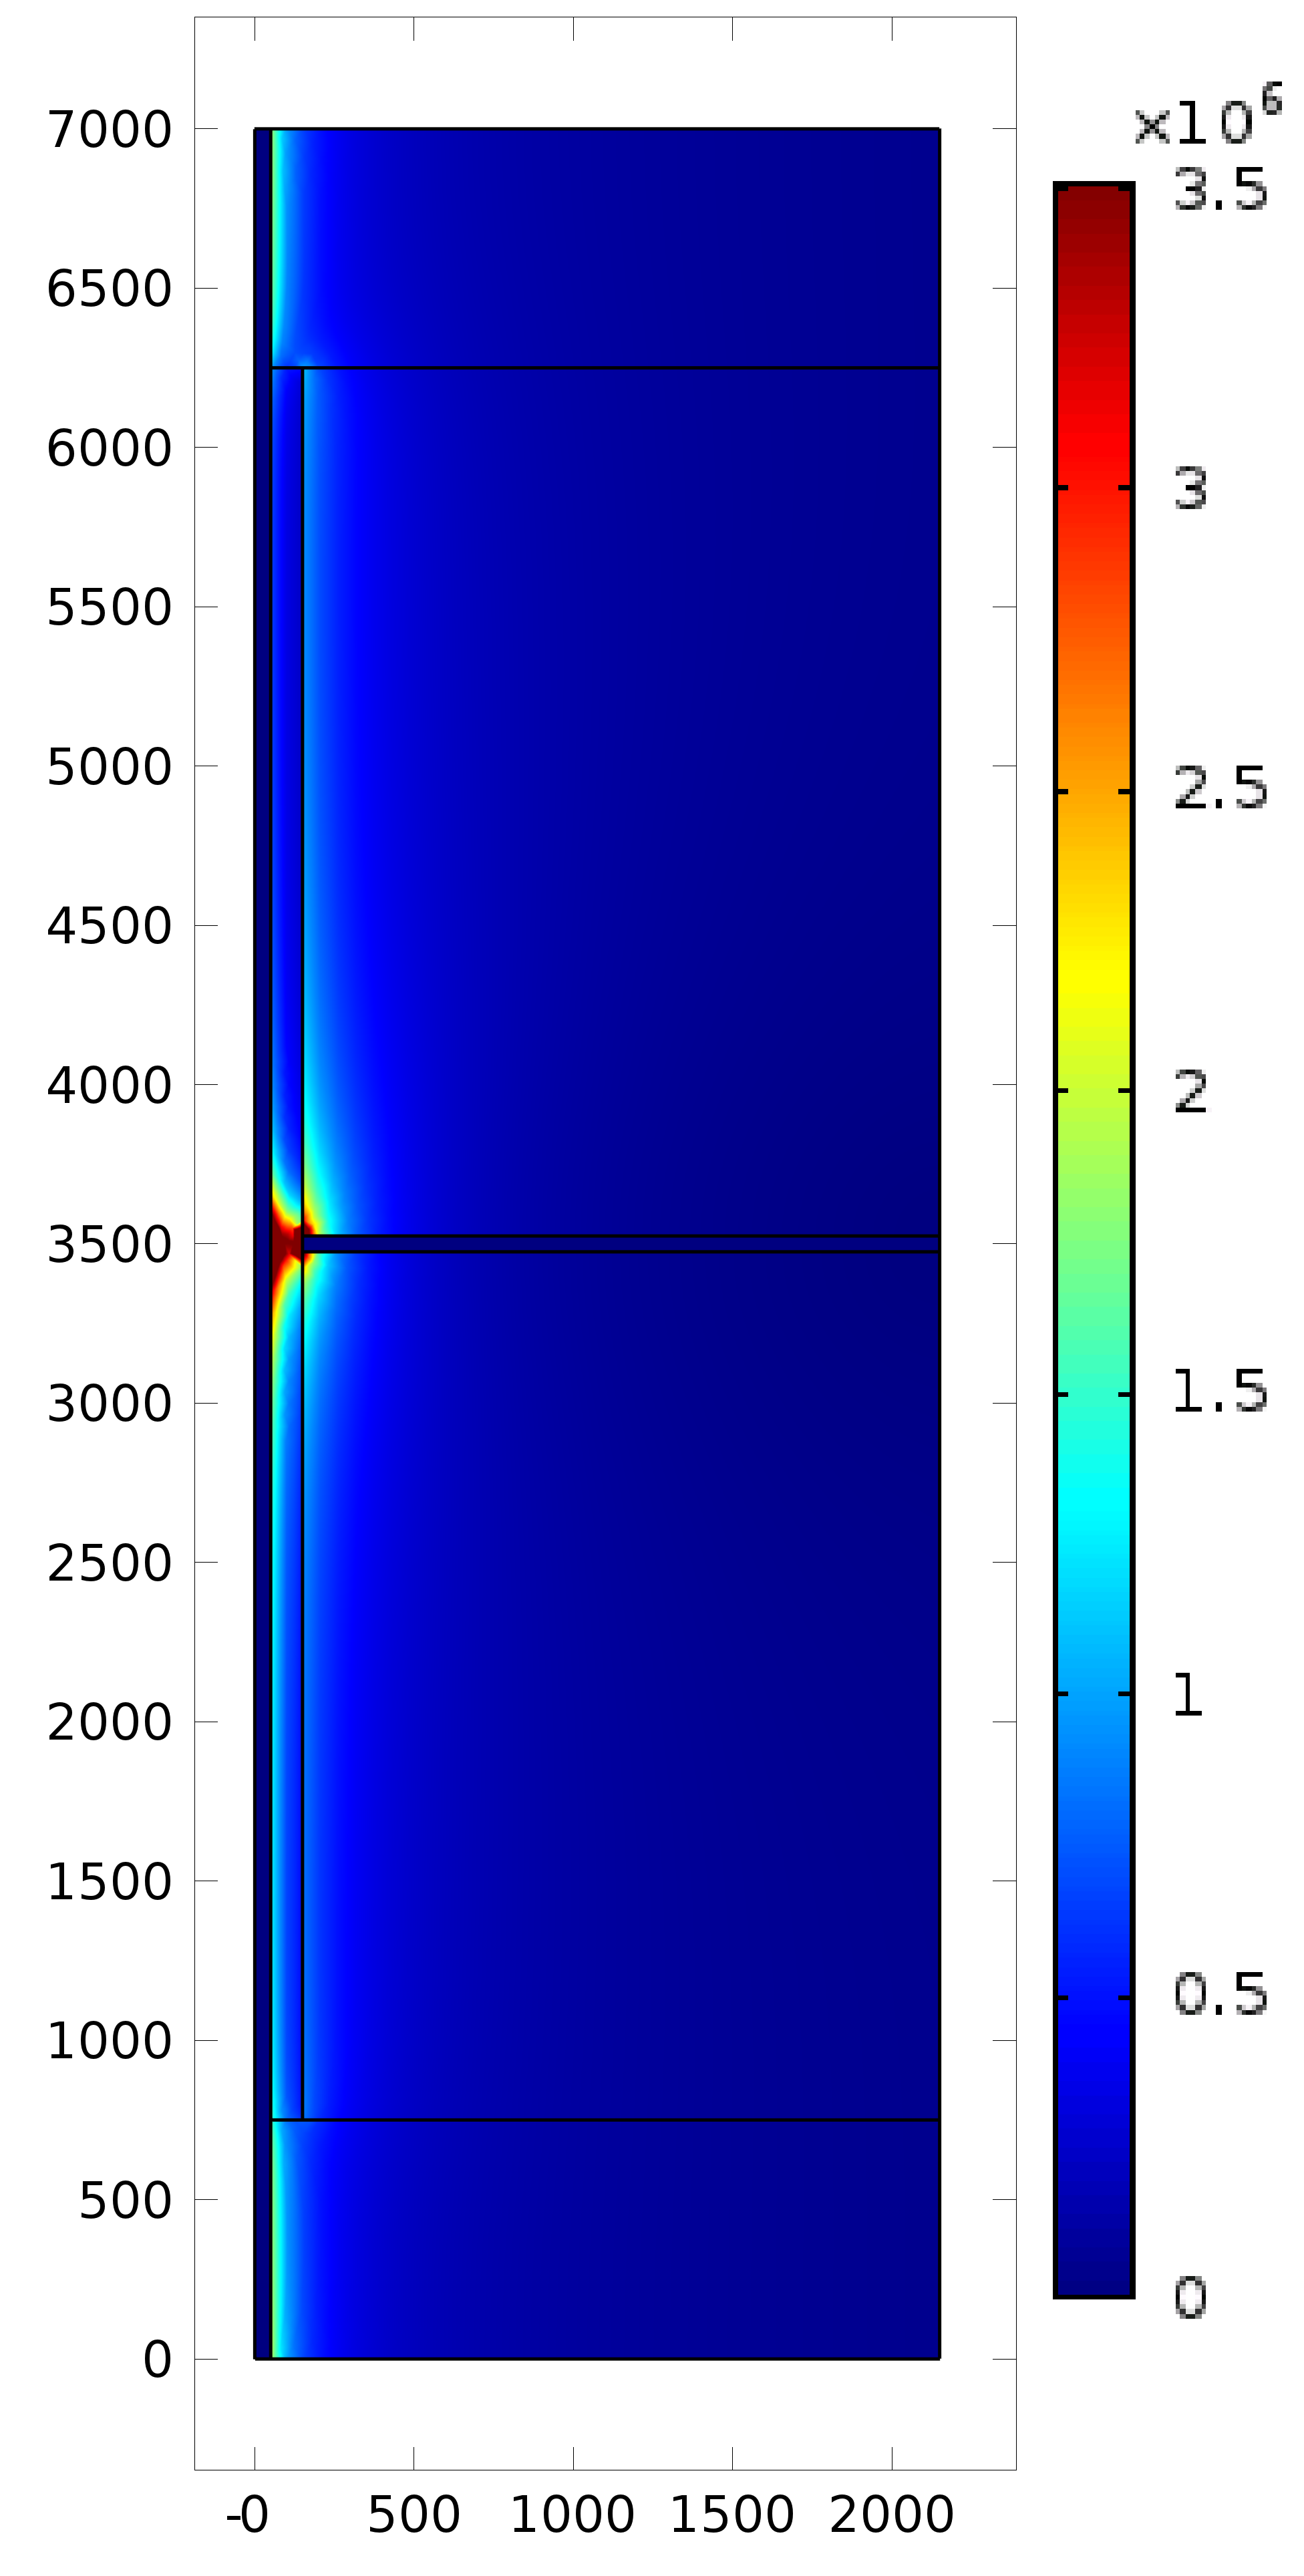
\includegraphics[width = 0.8\textwidth]{./Figures/Simulations/Edited_No_Foils_Large/Norm_E_Field.eps} 
\caption{Normal Electric Field (V/m) for Baseline Model}
\label{Figure:No_Foil_Large_Field}
\end{figure}

The air and oil extends radially 2m from the end of the bushing and 1m in the axial direction.
This is to understand the anticipated area of interest in the model.
By considering figure \ref{Figure:No_Foil_Large_Field} it is clear that there is very little happening further than 500mm radially from the bushing surface and there is very little of interest further than 200mm in the axial direction.
Therefore all further models will adhere to this geometry, ensuring that the area of interest is captured, while decreasing simulation times to a minimum.

In figure \ref{Figure:No_Foil_Large_Field}, the normal electric field throughout the whole system is displayed.
Electric field is usually taken to be a vector quantity, that is a magnitude and direction. 
For example, the electric field in the radial direction is termed $E_r$ and in the axial direction is $E_z$.
The normal electric field is not a normal vector, but an absolute value of the electric field strength at a given point. 
This can be described mathematically as $normE = \sqrt{\mathbf{E}.\mathbf{E}}$.
It gives a reasonable interpretation of the electric field strength in either vector direction in the model, and will be used to compare all other models.

\subsection{No Foils}
In order to illustrate the requirement for capacitive grading within AC bushings, a simulation of a bushing with no foils was conducted.
Figure \ref{Figure:No_Foil_Geom} shows the geometry and materials used for each section.
The conductor length is $6000mm$ and has a width of half the inner diameter, $50mm$. 
The paper impregnated with oil insulation is $5500mm$ long in order to accommodate the first foil length of $5000mm$ with sufficient clearance. 
The transformer wall is modelled as a $50mm$ high aluminium block that is $500mm$ wide, and is placed vertically in the middle of the design. The surrounding oil and air are $500mm$ wide at the centre of the bushing, and extend to the length of the conductor.
The paper impregnated with oil insulation is sloped to avoid sharp corners and high field strengths.
\begin{figure}[!h]
  \centering
    \includegraphics[width = \textwidth]{./Figures/Simulations/Edited_No_Foils_Final/Geometry.eps} 
	\caption{Geometry and Materials for No Foils Bushing}
\label{Figure:No_Foil_Geom}
\end{figure}


A very fine mesh was used in this model as shown in figure \ref{Figure:No_Foil_Mesh}. This allows for the maximum level of accuracy in the results produced, and is possible since the geometry of this model is not over-complex. It was necessary to ensure the mesh in the plane of the transformer wall was very fine in order to sufficiently capture areas of very high field.
\begin{figure}[!h]
  \centering
    \includegraphics[width = \textwidth]{./Figures/Simulations/Edited_No_Foils_Final/No_Foils_Mesh_Wide.eps} 
	\caption{Extra Fine Mesh for No Foils Bushing}
\label{Figure:No_Foil_Mesh}
\end{figure}


\begin{figure}[!h]
  \centering
    \includegraphics[width = \textwidth]{./Figures/Simulations/Edited_No_Foils_Final/No_Foils_E_Field_Norm_Wide.eps} 
	\caption{Normal Electric Field (V/m) for No Foils Bushing}
\label{Figure:No_Foil_Field}
\end{figure}


The motivation for capacitive grading is clear in figure \ref{Figure:No_Foil_Field}. 
The central area of stress in the plane of the transformer wall is shown in figure \ref{figure:problemfield}.
The highest stress is shown at the corners of the transformer wall and in the plane between the transformer wall and the conductor.
This reaches field strengths greater than $4.5kV/mm$ which can cause the inception of partial discharge.
This simulation bears close resemblance to figure \ref{figure:problem} in section \ref{s:method} of this report, which was used to describe the electric field problem.
In order for this bushing to function within the design constraints, capacitive grading must be used.

\begin{figure}[!h]
   \centering
   \includegraphics[width = 0.5\textwidth]{./Figures/Simulations/Edited_No_Foils_Final/No_Foils_E_Field_Norm_Close.eps}
   \caption{Area of very high electric stress}
   \label{figure:problemfield}
\end{figure}

\subsection{No Grading} \label{ss:no_grading}
In order to rectify the high electric stress identified in the no foils model, isolated foils are introduced to capacitively grade the electric field.
To prove the requirement for grading the lengths or radial displacement of the foils, a simulation where the foils are maintained at the same length was performed.
This model was expected to fail the design criteria, proving that introducing isolated foils into the bushing achieves very little and it is the radial or axial grading of the field that is critical.
The bushing has 21 foils spaced at an even radial spacing, but with no change in length of each foil.
Each foil is $1756mm$ in length, and is centred in the within the bushing. 

\begin{figure}[!h]
  \centering
    \includegraphics[width = \textwidth]{./Figures/Simulations/Edited_No_Grading_Final/Geometry.eps} 
	\caption{Geometry of the No Grading Model}
	\label{Figure:No_Grading_Geom}
\end{figure}

Producing a finite element mesh for this model caused issues with long computation time. 
Even using the coarsest default setting, the meshing time was of the order of days.
This is due to the difference in size of the aspects of the geometry.
The foils are just $0.1mm$ thick, which requires a very small set of triangles in order to mesh this area.
The other domains are up to $6000mm$ long, which is considerably larger and requires a different size of triangles.

\begin{figure}[!h]
  \centering
    \includegraphics[width = \textwidth]{./Figures/Simulations/Edited_No_Grading_Final/Mesh_wide.eps} 
	\caption{User defined meshing for no grading simulation - whole view}
\label{Figure:No_Grading_Mesh1}
\end{figure}

In order to solve the issue, a set of meshing rules were produced.
Firstly, the mesh within the conductor and within the foils can be very coarse.
Within a conducting material, no electric field is expected, hence there is no reason to finely mesh that area.
Areas of interest or areas where the field changes rapidly need to have a very fine mesh to ensure the accuracy of the results is sufficient.
The meshing rules dictated a minimum number of points at the tip of each foil, and along the surface of the bushing.
This resulted in a refined mesh shown in figures \ref{Figure:No_Grading_Mesh1} and \ref{Figure:No_Grading_Mesh2}.

\begin{figure}[!h]
  \centering
    \includegraphics[width = 0.4\textwidth]{./Figures/Simulations/Edited_No_Grading_Final/Mesh_Close.eps} 
	\caption{User defined meshing for no grading simulation - foil tip view}
\label{Figure:No_Grading_Mesh2}
\end{figure}

Once the geometry has been meshed appropriately, the system can be solved to determine the electric field strength throughout the model, as shown in figure \ref{Figure:No_Grading_Fieldxy}.


\begin{figure}[!h]
  \centering
   \subfigure[Normal Electric Field (V/m) for the No-Grading Model]{
    \includegraphics[width = \textwidth]{./Figures/Simulations/Edited_No_Grading_Final/E_Field_Norm_Wide.eps} 
	%\caption{Normal Electric Field (V/m) for the No-Grading Model - Whole view}
	\label{Figure:No_Grading_Field_Wide}
   }\\

\subfigure[Normal Electric Field (V/m) in the Plane of the Transformer Wall]{
    \includegraphics[width = 0.42\textwidth]{./Figures/Simulations/Edited_No_Grading_Final/E_Field_Norm_Close_Mid.eps} 
	%\caption{Normal Electric Field (V/m) for the No-Grading Model}
	\label{Figure:No_Grading_Field_CloseMid}
   } \quad
\subfigure[Normal Electric Field (V/m) at the tips of the Foils]{
    \includegraphics[width = 0.48\textwidth]{./Figures/Simulations/Edited_No_Grading_Final/E_Field_Norm_Close_Tip.eps} 
	%\caption{Normal Electric Field (V/m) for the No-Grading Model}
	\label{Figure:No_Grading_Field_CloseTip}
   }
\caption{Examination of the Electric Field in the Non-Grading Model}
\label{Figure:No_Grading_Fieldxy}
\end{figure}

Figure \ref{Figure:No_Grading_Field_CloseMid} shows the normal electric field in the plane of the transformer wall. 
The areas of very high field at the corners of the transformer wall have been eliminated by the use of the capacitive foils.
However, the field close to the conductor is still very high.
An additional issue is introduced by using capacitive foils.
Considering figure \ref{Figure:No_Grading_Field_CloseTip}, the tips of the foils cause some considerable disturbance of the electric field.
This model achieves very little improvement, if at all, over the model with no foils.

Now that the requirement for grading has been shown in section \ref{ss:no_grading}, and the requirement to use a formal axial or radial grading method in this section, the radial and axial designs can be compared.


\subsection{Radial Grading}
The COMSOL geometry for the radial grading model is shown figure \ref{Figure:Radial_Geom}. 
Each foil is an equal radial distance according to the radial grading method.
The lengths of each foil are taken from table \ref{table:radialvals}.
The remainder of the geometry is identical to the No Foils and No Grading models.

\begin{figure}[!h]
  \centering
    \includegraphics[width = \textwidth]{./Figures/Simulations/Edited_Radial_Final/Geometry.eps} 
	\caption{Geometry of the Radial Model}
	\label{Figure:Radial_Geom}
\end{figure}

As with the No Grading model, the geometry in this design is very complex with a variety of scales.
In order to reduce computation time but maintain a reasonable level of accuracy in areas of interest, the mesh was produced to the rules outlined for the No Grading model. The meshing for this model is shown in figure \ref{Figure:Radial_Mesh_wide} and \ref{Figure:Radial_Mesh_close}. 
\begin{figure}[!h]
  \centering
    \includegraphics[width = \textwidth]{./Figures/Simulations/Edited_Radial_Final/Radial_Mesh_Wide.eps} 
	\caption{Meshing of the Radial Model}
	\label{Figure:Radial_Mesh_wide}
\end{figure}

\begin{figure}[!h]
  \centering
    \includegraphics[width = 0.7\textwidth]{./Figures/Simulations/Edited_Radial_Final/Radial_Mesh_Close.eps} 
	\caption{Meshing of the Radial Model Focused on a Foil Tip}
	\label{Figure:Radial_Mesh_close}
\end{figure}

The model was then solved to find the normal electric field throughout the model.
It can be seen in figure \ref{Figure:Radial_Field_CloseMid} that the field between the foils nearest the conductor is reduced below $4.5kV/mm$.
This is now evenly spread in the radial direction, as expected due to the radial grading of the electric field.
The electric field in the radial direction is much improved.

However, the axial electric field is not considered in the radial grading design method.
The field at the foil tips is largely due to the axial field strength.
It is necessary to inspect the strength of the electric fields at the tips of the foils.
It can be seen in figure \ref{Figure:Radial_Field_CloseTip} that the electric field at the tips of the foil exceeds $4.5kV/mm$ in some places.
Section \ref{s:Discussion} will take this observation further, to establish if it meets the design criteria.

\begin{figure}[!h]
  \centering
   %\subfigure[Normal Electric Field (V/m) for the No-Grading Model]{
    \includegraphics[width = \textwidth]{./Figures/Simulations/Edited_Radial_Final/Radial_E_Field_Norm_Wide.eps} 
	\caption{Normal Electric Field (V/m) for the Radial - Whole view}
	\label{Figure:Radial_Field_Wide}
   \end{figure}

\begin{figure}[!h]
  \centering
\subfigure[Normal Electric Field (V/m) in the Plane of the Transformer Wall]{
    \includegraphics[width = 0.45\textwidth]{./Figures/Simulations/Edited_Radial_Final/E_Field_Norm_Middle.eps} 
	%\caption{Normal Electric Field (V/m) for the No-Grading Model}
	\label{Figure:Radial_Field_CloseMid}
   } 
\subfigure[Normal Electric Field (V/m) at the tips of the Foils]{
    \includegraphics[width = 0.45\textwidth]{./Figures/Simulations/Edited_Radial_Final/Radial_E_Field_Norm_Close_Tip.eps} 
	%\caption{Normal Electric Field (V/m) for the No-Grading Model}
	\label{Figure:Radial_Field_CloseTip}
   }
\caption{Examination of the Electric Field in the Radial Model}
\label{Figure:Radial_Field}
\end{figure}




\subsection{Axial Grading}
The asymmetric axial grading method results in an uneven geometry about the centre of the bushing.
The lengths of each foil is determined in table \ref{table:axialvals}.
This requires the paper insulation to take a different profile than the other models in order to adequately cover the foils, as shown in figure \ref{Figure:Axial_Geom}.
The air side has a much longer surface area due to the higher creepage distance of air.
\begin{figure}[!h]
  \centering
    \includegraphics[width = \textwidth]{./Figures/Simulations/Edited_Axial_Final/Geometry.eps} 
	\caption{Geometry of the Axial Model}
	\label{Figure:Axial_Geom}
\end{figure}

The meshing for this model follows the design rules, in order to produce the finest mesh over the key points of interest, shown in figure \ref{Figure:Axial_Mesh_wide}.
Particularly figure \ref{Figure:Axial_Mesh_close} shows the fine mesh around the tip of a foil, which is a key area of interest to determine if the PD inception condition is maintained.
\begin{figure}[!h]
  \centering
    \includegraphics[width = \textwidth]{./Figures/Simulations/Edited_Axial_Final/Axial_Mesh_Wide.eps} 
	\caption{Meshing of the Axial Model}
	\label{Figure:Axial_Mesh_wide}
\end{figure}

\begin{figure}[!h]
  \centering
    \includegraphics[width = 0.4\textwidth]{./Figures/Simulations/Edited_Axial_Final/Axial_Mesh_Close.eps} 
	\caption{Meshing of the Axial Model Focused on a Foil Tip}
	\label{Figure:Axial_Mesh_close}
\end{figure}

The electric field problem can now be solved over the whole model.
This produces the surface plots shown in figures \ref{Figure:Radial_Field_Wide} and \ref{Figure:No_Grading_Field}.
It can be seen that the field in the plane of the transformer wall is not well graded, as it is neglected in the axial design method.
The field at the foil tips for which the main contributor is the axial field has a smaller area exposed to high field strengths than the radial method.
However, it remains an issue to be considered.
This will be discussed and contrasted with the other designs in the discussion in section \ref{s:Discussion}.

\begin{figure}[!h]
  \centering
   %\subfigure[Normal Electric Field (V/m) for the No-Grading Model]{
    \includegraphics[width = \textwidth]{./Figures/Simulations/Edited_Axial_Final/E_Field_Norm_Wide.eps} 
	\caption{Normal Electric Field (V/m) for the Axial Model - Whole view}
	\label{Figure:Radial_Field_Wide}
   \end{figure}

\begin{figure}[!h]
  \centering
\subfigure[Normal Electric Field (V/m) in the Plane of the Transformer Wall]{
    \includegraphics[width = 0.45\textwidth]{./Figures/Simulations/Edited_Axial_Final/E_Field_Norm_Mid.eps} 
	%\caption{Normal Electric Field (V/m) for the No-Grading Model}
	\label{Figure:Radial_Field_CloseMid}
   } 
\subfigure[Normal Electric Field (V/m) at the tips of the Foils]{
    \includegraphics[width = 0.45\textwidth]{./Figures/Simulations/Edited_Axial_Final/Axial_E_Field_Norm_Close_Tip.eps} 
	%\caption{Normal Electric Field (V/m) for the No-Grading Model}
	\label{Figure:Radial_Field_CloseTip}
   }
\caption{Examination of the Electric Field in the Axial Model}
\label{Figure:No_Grading_Field}
\end{figure}

%\clearpage 

%\subsection{No Grading}
%As a baseline for comparison, a bushing with no foils has been constructed and simulated.
%The geometry of the model was built as in figure \ref{figure:Geom:Nograde}.
%The system is an axialsymmetric 2D model, which takes the central vertical point $r=0$ as the centre of a cylinder.
%\begin{figure}[!h]
%   \centering
%   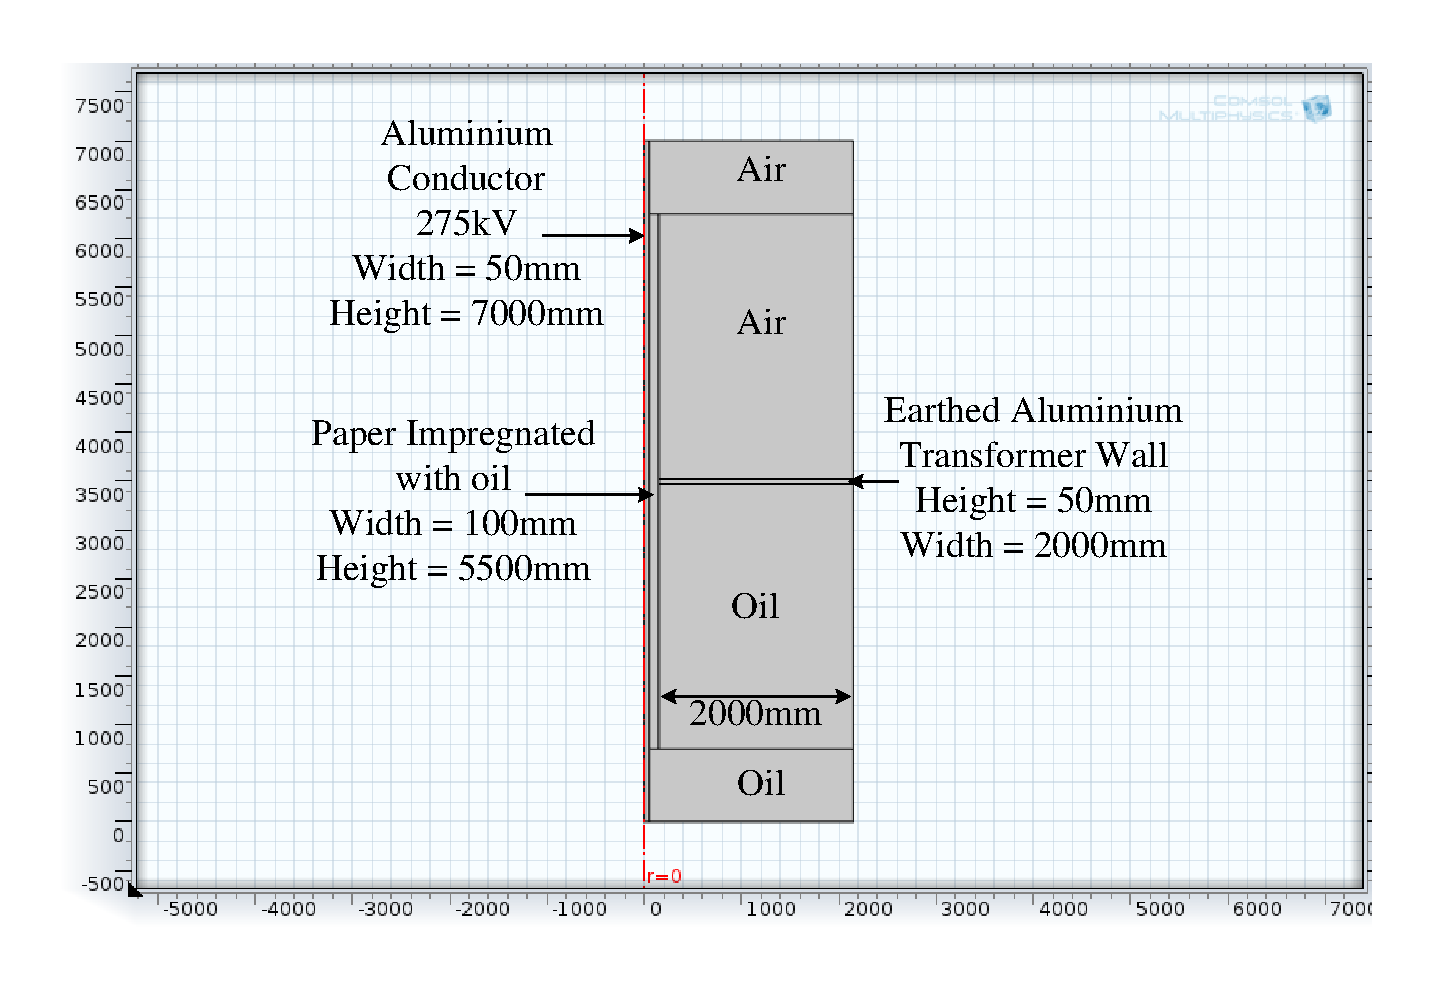
\includegraphics[width = 0.8\textwidth]{NoGradingBlock.pdf}
%   \caption{COMSOL Geometry Annotated with Materials - No Grading}
%   \label{figure:Geom:Nograde}
%\end{figure}
%
%Once the geometry of the model is defined, a finite element mesh can be created as shown in figure \ref{figure:Mesh:Nograde}.
%This model is fairly simple, hence a very fine graded mesh was used improving the accuracy of results.
%\begin{figure}[!h]
%   \centering
%   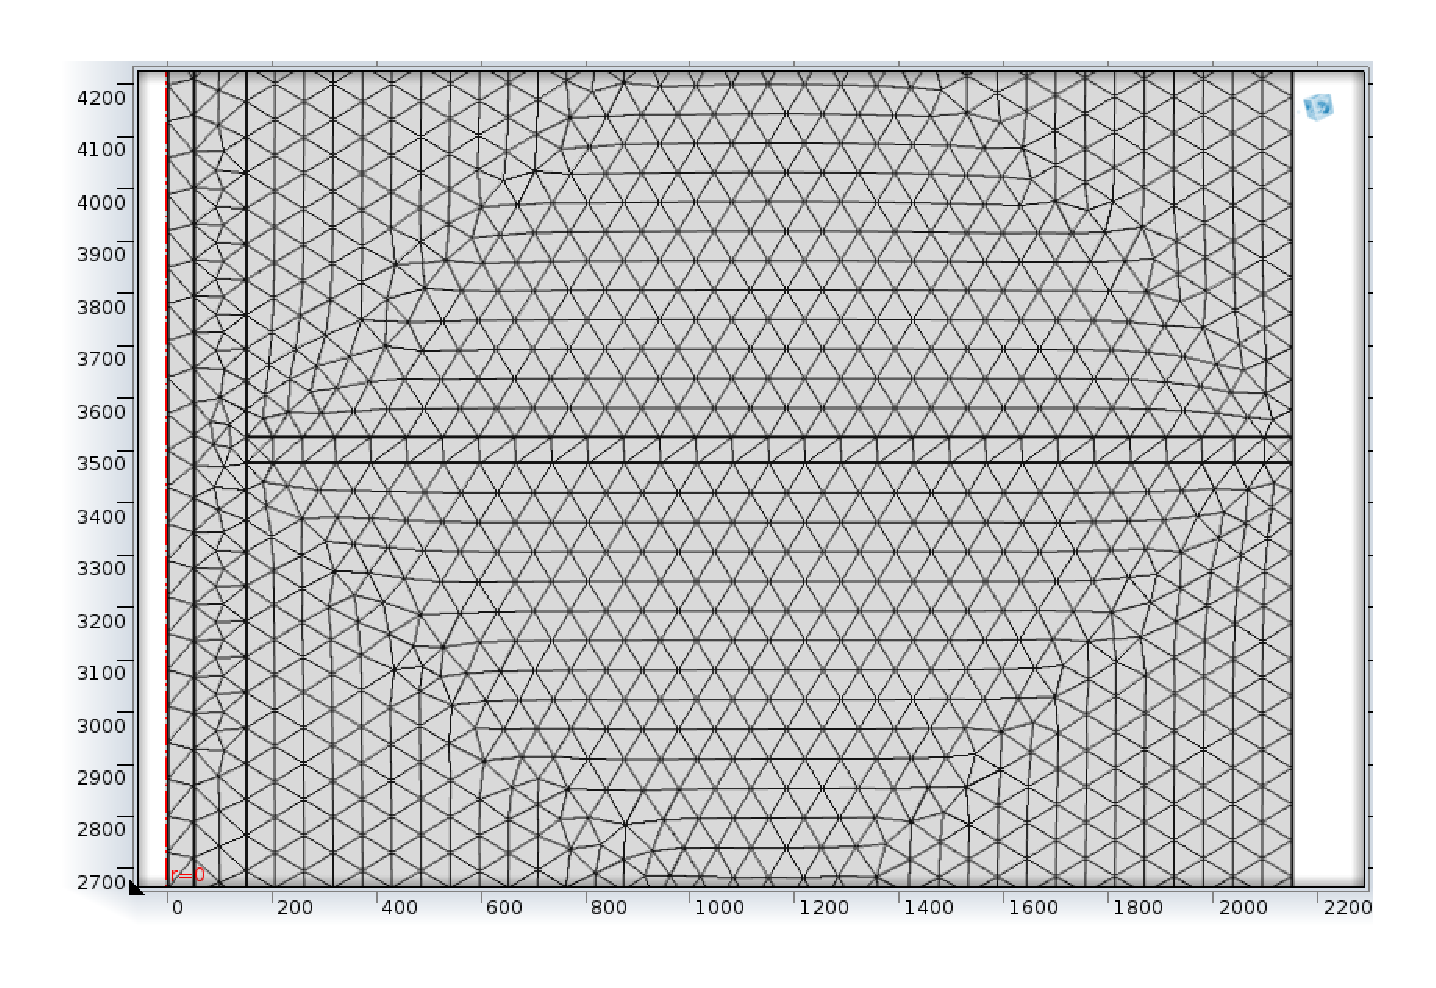
\includegraphics[width = 0.8\textwidth]{NoGradingMesh.pdf}
%   \caption{COMSOL Mesh - No Grading}
%   \label{figure:Mesh:Nograde}
%\end{figure}
%
%The next stage is to define the relative permittivity of each of the materials used for each sub section of the geometry.
%The initial conditions must then be set, with the conductor set to 275kV, and the transformer wall and all outer boundaries earthed.
%All other boundaries are assumed to be continuity boundaries.
%
%The model can then be solved to give the electric field distribution
%\inote{TS - Report done up to here 03/03/2014}
.
%\begin{figure}[!h]
%   \centering
%   \includegraphics[width = 0.8\textwidth]{WideNoGrading.png}
%\end{figure}
%
%\begin{figure}[!h]
%   \centering
%   \includegraphics[width = 0.8\textwidth]{CloseNoGrading.png}
%\end{figure}
%
%\begin{figure}[!h]
%   \centering
%   \includegraphics[width = 0.8\textwidth]{SurfaceGraded21.png}
%\end{figure}
%
%\begin{figure}[!h]
%   \centering
%   \includegraphics[width = 0.8\textwidth]{WideGraded21.png}
%\end{figure}
%
%\begin{figure}[!h]
%   \centering
%   \includegraphics[width = 0.8\textwidth]{CloseGraded21.png}
%\end{figure}
%
%\begin{figure}[!h]
%   \centering
%   \includegraphics[width = 0.8\textwidth]{SurfaceGradedCloseish21.png}
%\end{figure}